\documentclass{llncs}
\usepackage{graphicx}
\begin{document}
  \title{A Method to Protect the Security of Your Smart-phone}
  \author{Yu Zhuolong\inst{1} \and Guo Hansong\inst{2}}
  \institute{University of Science and Technology of China}
  \maketitle
  %
  \begin{abstract}
    As utility of smart-phone arises, the security of smart-phone has become a.
  \end{abstract}
  %
  \section{Fixed-Period Problems: The Sublinear Case}
  %
  With this chapter, the preliminaries are over, and we begin the search for periodic solutions \dots
  %
  \subsection{Autonomous Systems}
  %
  In this section we will consider the case when the Hamiltonian $H(x)$ \dots
  %
  \subsubsection{The General Case: Nontriviality.}
  %
  We assume that $H$ is
  $\left(A_{\infty}, B_{\infty}\right)$-subqua\-dra\-tic at infinity, for some constant \dots
  %
  \paragraph{Notes and Comments.}
  The first results on subharmonics were \dots
  %
  \begin{proposition}
    Assume $H'(0)=0$ and $ H(0)=0$. Set \dots
  \end{proposition}
  
  \begin{figure}
    %\vspace{2.5cm}
    \begin{center}
    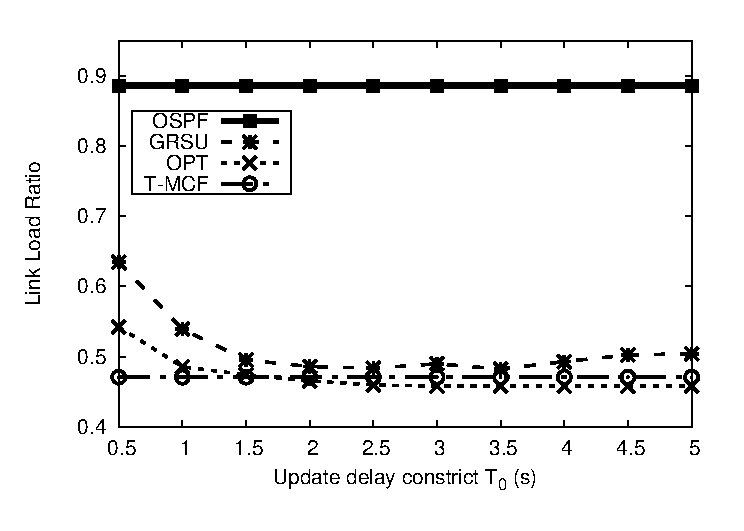
\includegraphics[height=2.5cm]{12.eps}
    \end{center}
    \caption{This is a figure.}
  \end{figure}
  
  
  \begin{proof}[of proposition]
    Condition (8) means that, for every \LaTeX $\delta'>\delta$, the some $\varepsilon>0$ such that \dots \qed
  \end{proof}
  %
  \begin{example}[\rmfamily (External forcing)]
    Consider the system \dots
  \end{example}
  
  
  \begin{corollary}
    Assume $H$ is $C^{2}$ end
    $\left(a_{\infty}, b_{\infty}\right)$-subquadratic at infinity. Let \dots
  \end{corollary}
  \begin{lemma}
    Assume that $H$ is $C^{2}$ on $\bbbr^{2n}\backslash \{0\}$ and that $H''(x)$ is \cite{clar:eke}\dots
  \end{lemma}
  \begin{theorem}[Ghoussoub-Preiss]
    Let $X$ be a Banach Space and $\Phi:X\to\bbbr$ \dots
  \end{theorem}
  
  \begin{definition}
    We shall say that a $C^{1}$ function \footnote{The footnote is automatically numbered.} $\Phi:X\to\bbbr$ satisfies \dots
  \end{definition}
  
  \begin{thebibliography}{1}
    \bibitem{clar:eke}
    Clarke, F., Ekeland, I.:
    Nonlinear oscillations and  boundary-value problems for Hamiltonian systems
    Arch. Rat. Mech. Anal. 78, 315--333(1982)
  \end{thebibliography}
  %\begin{equation}
    %\left(\frac{a^{2} + b^{2}}{c^{3}} \right) = 1 \quad
    %\mbox{ if } c\neq 0 \mbox{ and if | a,b,c\in \bbbr \enspace
    
  %\end{equation}
  
\end{document}
